\documentclass[a4paper,11pt]{article}
\usepackage[utf8]{inputenc}
\usepackage{amssymb}
\usepackage{amsmath} 
\usepackage{enumerate}
\usepackage{tikz}

\DeclareMathOperator*{\argmax}{arg\!\max}
\DeclareMathOperator*{\argmin}{arg\!\min}
\DeclareMathOperator*{\doop}{do}
\DeclareMathOperator*{\var}{var}
\newcounter{exercise}
\setcounter{exercise}{0}
\newcounter{subexercise}
\newcommand*{\exercise}[1][]{
  \subsection*{Exercise
    \ifx/#1/\stepcounter{exercise}\arabic{exercise}
    \else#1\fi
  }
  \setcounter{subexercise}{0}
}
\newcommand*{\subexercise}[1][]{
  \par{
    \noindent{\ifx/#1/\protect\stepcounter{subexercise}\alph{subexercise}\else#1\fi.\quad}
  }
}
\title{Chapter 26}
\author{stevenjin8}
\date{July 11, 2021}

\begin{document}
	\maketitle

	\section*{Comments and Proofs}
	\section*{Exercises}
	\exercise
	\subexercise
	By conditioning on $\text{do}( S=T )$, the graph becomes
	\begin{center}
	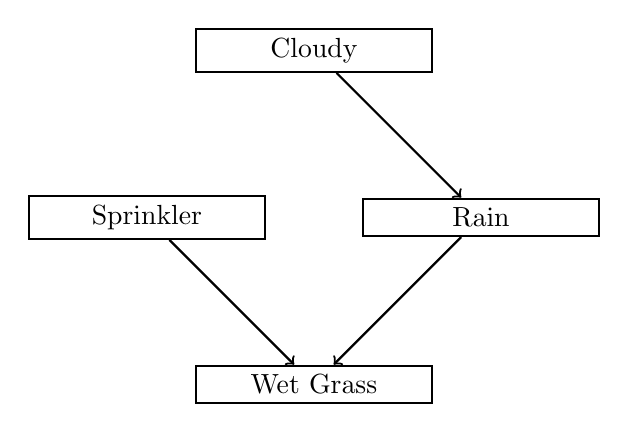
\begin{tikzpicture}[node distance={30mm}, thick, main/.style = {draw, minimum width=30mm}]
	  \node[main] (1) {Cloudy}; 
	  \node[main] (2) [below left of=1] {Sprinkler}; 
	  \node[main] (3) [below right of=1] {Rain};
	  \node[main] (4) [below right of=2] {Wet Grass};

	  \draw[->] (1) -- (3); 
	  \draw[->] (3) -- (4); 
	  \draw[->] (2) -- (4); 
	\end{tikzpicture}
	\end{center}
	The marginal for $R$ uniform (but if we were in Vancouver, $p(R=T)=1$). Thus,
	\begin{align*}
		p( W=T | \doop( S=T )) &= p( W=T, R=T | \doop( S=T )) + p( W=T, R=F | \doop( S=T )) \\
		&= p( W=T | R=T, \doop( S=T )) p( R=T | \doop( S=T )) \\
		& \qquad + p( W=T | R=F, \doop( S=T )) p( R=F | \doop( S=T ))) \\
		&= p( W=T | R=T, \doop( S=T )) p( R=T )\\
		&\qquad + p( W=T | R=F, \doop( S=T )) p( R=F ) \\
		&= 0.9 \times 0.5 + 0.99 \times 0.5 \\
		&= 0.945.
	\end{align*}

	\subexercise
	Similarly to part a, we have 
	\begin{align*}
		p( W=T | \doop( S=F )) &= p( W=T | R=T, \doop( S=F )) p( R=T )\\
		&\qquad + p( W=T | R=F, \doop( S=F )) p( R=F ) \\
		&= 0 \times 0.5 + 0.9 \times 0.5 \\
		&= 0.45.
	\end{align*}

	\subexercise
	Since $C$ is the root of the DAG, performing do-calculus makes no difference. Thus
	\[
	p( S=T | \doop( C=T ) ) = p( S=T | C=T ) = 0.1.
	\]
	Unsurprisingly, we find out that sprinklers cause grass to become wet.
\end{document}

